%% abtex2-modelo-trabalho-academico.tex, v-1.9.7 laurocesar
%% Copyright 2012-2018 by abnTeX2 group at http://www.abntex.net.br/ 
%%
%% This work may be distributed and/or modified under the
%% conditions of the LaTeX Project Public License, either version 1.3
%% of this license or (at your option) any later version.
%% The latest version of this license is in
%%   http://www.latex-project.org/lppl.txt
%% and version 1.3 or later is part of all distributions of LaTeX
%% version 2005/12/01 or later.
%%
%% This work has the LPPL maintenance status `maintained'.
%% 
%% The Current Maintainer of this work is the abnTeX2 team, led
%% by Lauro César Araujo. Further information are available on 
%% http://www.abntex.net.br/
%%
%% This work consists of the files abntex2-modelo-trabalho-academico.tex,
%% abntex2-modelo-include-comandos and abntex2-modelo-references.bib
%%

% ------------------------------------------------------------------------
% ------------------------------------------------------------------------
% abnTeX2: Modelo de Trabalho Academico (tese de doutorado, dissertacao de
% mestrado e trabalhos monograficos em geral) em conformidade com 
% ABNT NBR 14724:2011: Informacao e documentacao - Trabalhos academicos -
% Apresentacao
% ------------------------------------------------------------------------
% ------------------------------------------------------------------------

\documentclass[
% -- opções da classe memoir --
12pt,				% tamanho da fonte
openright,			% capítulos começam em pág ímpar (insere página vazia caso preciso)
twoside,			% para impressão em recto e verso. Oposto a oneside
a4paper,			% tamanho do papel. 
% -- opções da classe abntex2 --
%chapter=TITLE,		% títulos de capítulos convertidos em letras maiúsculas
%section=TITLE,		% títulos de seções convertidos em letras maiúsculas
%subsection=TITLE,	% títulos de subseções convertidos em letras maiúsculas
%subsubsection=TITLE,% títulos de subsubseções convertidos em letras maiúsculas
% -- opções do pacote babel --
english,			% idioma adicional para hifenização
french,				% idioma adicional para hifenização
spanish,			% idioma adicional para hifenização
brazil				% o último idioma é o principal do documento
]{abntex2}

% ---
% Pacotes básicos 
% ---
\usepackage{lmodern}			% Usa a fonte Latin Modern			
\usepackage[T1]{fontenc}		% Selecao de codigos de fonte.
\usepackage[utf8]{inputenc}		% Codificacao do documento (conversão automática dos acentos)
\usepackage{indentfirst}		% Indenta o primeiro parágrafo de cada seção.
\usepackage{color}				% Controle das cores
\usepackage{graphicx}			% Inclusão de gráficos
\usepackage{microtype} 			% para melhorias de justificação
% ---

% ---
% Pacotes adicionais, usados apenas no âmbito do Modelo Canônico do abnteX2
% ---
\usepackage{lipsum}				% para geração de dummy text
% ---

% ---
% Pacotes de citações
% ---
\usepackage[brazilian,hyperpageref]{backref}	 % Paginas com as citações na bibl
\usepackage[alf]{abntex2cite}	% Citações padrão ABNT

% --- 
% CONFIGURAÇÕES DE PACOTES
% --- 

% ---
% Configurações do pacote backref
% Usado sem a opção hyperpageref de backref
\renewcommand{\backrefpagesname}{Citado na(s) página(s):~}
% Texto padrão antes do número das páginas
\renewcommand{\backref}{}
% Define os textos da citação
\renewcommand*{\backrefalt}[4]{
	\ifcase #1 %
	Nenhuma citação no texto.%
	\or
	Citado na página #2.%
	\else
	Citado #1 vezes nas páginas #2.%
	\fi}%
% ---

% ---
% Informações de dados para CAPA e FOLHA DE ROSTO
% ---
\titulo{Classificando Políticos Autoritários: uma prova de conceito com a Câmara dos Deputados no Brasil}
\autor{Marcio de Lucas Cunha Gomes}
\local{Brasil}
\data{2020}
\orientador{Nara Pavão}
\coorientador{}
\instituicao{%
	Universidade Federal de Pernambuco -- UFPE
	\par
	Departamento de Ciência Política
	\par
	Programa de Pós-Graduação}
\tipotrabalho{Dissertação (Mestrado)}
% O preambulo deve conter o tipo do trabalho, o objetivo, 
% o nome da instituição e a área de concentração 
\preambulo{Dissertação apresentada ao Departamento de Ciência Política da Universidade  Federal de Pernambuco para obtenção  do  título  de  Mestre em Ciência Política. Orientador: Prof. Dra. Nara Pavão}
% ---


% ---
% Configurações de aparência do PDF final

% alterando o aspecto da cor azul
\definecolor{blue}{RGB}{41,5,195}

% informações do PDF
\makeatletter
\hypersetup{
	%pagebackref=true,
	pdftitle={\@title}, 
	pdfauthor={\@author},
	pdfsubject={\imprimirpreambulo},
	pdfcreator={LaTeX with abnTeX2},
	pdfkeywords={abnt}{latex}{abntex}{abntex2}{trabalho acadêmico}, 
	colorlinks=true,       		% false: boxed links; true: colored links
	linkcolor=blue,          	% color of internal links
	citecolor=blue,        		% color of links to bibliography
	filecolor=magenta,      		% color of file links
	urlcolor=blue,
	bookmarksdepth=4
}
\makeatother
% --- 

% ---
% Posiciona figuras e tabelas no topo da página quando adicionadas sozinhas
% em um página em branco. Ver https://github.com/abntex/abntex2/issues/170
\makeatletter
\setlength{\@fptop}{5pt} % Set distance from top of page to first float
\makeatother
% ---

% ---
% Possibilita criação de Quadros e Lista de quadros.
% Ver https://github.com/abntex/abntex2/issues/176
%
\newcommand{\quadroname}{Quadro}
\newcommand{\listofquadrosname}{Lista de quadros}

\newfloat[chapter]{quadro}{loq}{\quadroname}
\newlistof{listofquadros}{loq}{\listofquadrosname}
\newlistentry{quadro}{loq}{0}

% configurações para atender às regras da ABNT
\setfloatadjustment{quadro}{\centering}
\counterwithout{quadro}{chapter}
\renewcommand{\cftquadroname}{\quadroname\space} 
\renewcommand*{\cftquadroaftersnum}{\hfill--\hfill}

\setfloatlocations{quadro}{hbtp} % Ver https://github.com/abntex/abntex2/issues/176
% ---

% --- 
% Espaçamentos entre linhas e parágrafos 
% --- 

% O tamanho do parágrafo é dado por:
\setlength{\parindent}{1.3cm}

% Controle do espaçamento entre um parágrafo e outro:
\setlength{\parskip}{0.2cm}  % tente também \onelineskip

% ---
% compila o indice
% ---
\makeindex
% ---

% ----
% Início do documento
% ----
\begin{document}
	
	% Seleciona o idioma do documento (conforme pacotes do babel)
	%\selectlanguage{english}
	\selectlanguage{brazil}
	
	% Retira espaço extra obsoleto entre as frases.
	\frenchspacing 
	
	% ----------------------------------------------------------
	% ELEMENTOS PRÉ-TEXTUAIS
	% ----------------------------------------------------------
	% \pretextual
	
	% ---
	% Capa
	% ---
	\imprimircapa
	% ---
	
	% ---
	% Folha de rosto
	% (o * indica que haverá a ficha bibliográfica)
	% ---
	\imprimirfolhaderosto*
	% ---
	
	% ---
	% Inserir a ficha bibliografica
	% ---
	
	% Isto é um exemplo de Ficha Catalográfica, ou ``Dados internacionais de
	% catalogação-na-publicação''. Você pode utilizar este modelo como referência. 
	% Porém, provavelmente a biblioteca da sua universidade lhe fornecerá um PDF
	% com a ficha catalográfica definitiva após a defesa do trabalho. Quando estiver
	% com o documento, salve-o como PDF no diretório do seu projeto e substitua todo
	% o conteúdo de implementação deste arquivo pelo comando abaixo:
	%
	% \begin{fichacatalografica}
	%     \includepdf{fig_ficha_catalografica.pdf}
	% \end{fichacatalografica}

\begin{fichacatalografica}
\sffamily
\vspace*{\fill}					% Posição vertical
\begin{center}					% Minipage Centralizado
	\fbox{\begin{minipage}[c][8cm]{13.5cm}		% Largura
			\small
			\imprimirautor
			%Sobrenome, Nome do autor
			
			\hspace{0.5cm} \imprimirtitulo  / \imprimirautor. --
			\imprimirlocal, \imprimirdata-
			
			\hspace{0.5cm} \thelastpage p. : il. (algumas color.) ; 30 cm.\\
			
			\hspace{0.5cm} \imprimirorientadorRotulo~\imprimirorientador\\
			
			\hspace{0.5cm}
			\parbox[t]{\textwidth}{\imprimirtipotrabalho~--~\imprimirinstituicao,
				\imprimirdata.}\\
			
			\hspace{0.5cm}
			1. Palavra-chave1.
			2. Palavra-chave2.
			2. Palavra-chave3.
			I. Orientador.
			II. Universidade xxx.
			III. Faculdade de xxx.
			IV. Título 			
		\end{minipage}}
	\end{center}
\end{fichacatalografica}
% ---


% ---
% Inserir folha de aprovação
% ---

% Isto é um exemplo de Folha de aprovação, elemento obrigatório da NBR
% 14724/2011 (seção 4.2.1.3). Você pode utilizar este modelo até a aprovação
% do trabalho. Após isso, substitua todo o conteúdo deste arquivo por uma
% imagem da página assinada pela banca com o comando abaixo:
%
% \begin{folhadeaprovacao}
% \includepdf{folhadeaprovacao_final.pdf}
% \end{folhadeaprovacao}
%
\begin{folhadeaprovacao}
	
	\begin{center}
		{\ABNTEXchapterfont\large\imprimirautor}
		
		\vspace*{\fill}\vspace*{\fill}
		\begin{center}
			\ABNTEXchapterfont\bfseries\Large\imprimirtitulo
		\end{center}
		\vspace*{\fill}
		
		\hspace{.45\textwidth}
		\begin{minipage}{.5\textwidth}
			\imprimirpreambulo
		\end{minipage}%
		\vspace*{\fill}
	\end{center}
	
	Trabalho aprovado. \imprimirlocal, 01 de março de 2020:
	
	\assinatura{\textbf{\imprimirorientador} \\ Orientador} 
	\assinatura{\textbf{Professor} \\ Davi Cordeiro Moreira}
	\assinatura{\textbf{Professor} \\ Jakson Alves de Aquino}
	
	\begin{center}
		\vspace*{0.5cm}
		{\large\imprimirlocal}
		\par
		{\large\imprimirdata}
		\vspace*{1cm}
	\end{center}
	
\end{folhadeaprovacao}
% ---

% ---
% Dedicatória
% ---
\begin{dedicatoria}
	\vspace*{\fill}
	\centering
	\noindent
	\textit{Este trabalho é dedicado aos meus pais \\ que sempre apoiaram meus sonhos, mesmo \\ quando isso significou me mudar para \\ longe de casa.} \vspace*{\fill}
\end{dedicatoria}
% ---

% ---
% Agradecimentos
% ---
\begin{agradecimentos}
	Agradeço aos meus pais, à Jakson e à Davi.	
\end{agradecimentos}
% ---		

% ---
% RESUMOS
% ---

% resumo em português
\setlength{\absparsep}{18pt} % ajusta o espaçamento dos parágrafos do resumo
\begin{resumo}
	Como mensurar autoritarismo nas atitudes de políticos eleitos por regimes democráticos? Apesar inúmeros trabalhos na Ciência Política tratarem das causas e consequências da ascenção de lideranças autoritárias em regimes democráticos, ainda existem ferramentas limitadas para identificá-las. Como forma de preencher uma lacuna na literatura, essa dissertação propõem-se a apresentar um modelo de classificação de agentes autoritários baseado nos seus discursos. O classificador é inspirado nas Escalas F e RWA, propostas por Adorno e Altemeyer, repectivamente, e utiliza-se de Named-Entity Recognition e Sentiment de Analysis como técnicas para medir sentido e intensidade do valor atribuído a entidades típicas do discurso autoritário. Como prova de conceito, utilizou-se 420 mil falas de 3700 parlamentares da Câmara dos Deputados, realizadas nos anos de 2000 à 2019. Entre os resultados, identificou-se que, apesar de flutuações significativas ao longo das legislaturas, 2018 é marcado por um ano de expressivo aumento de atitude autoritárias. Também é possível confirmar expectativas da literatura de que as bancadas da Bala e da Bíblia concentram, em média, maior número de parlamentares autoritários.

	\textbf{Palavras-chave}: autoritarismo, discurso político, Câmara dos Deputados, análise de conteúdo, processamento de linguagem natural, reconhecimento de entidades nomeadas, análise de sentimentos.
\end{resumo}

% resumo em inglês
\begin{resumo}[Abstract]
	\begin{otherlanguage*}{english}
		How to measure authoritarianism in the attitudes of political politicians by democratic regimes? Despite the numbers of works in Political Science, these are causes and consequences of the rise of authoritarian authorities in democratic regimes, but there are still limited tools to identify them. As a way to fill a gap in the literature, this dissertation proposed to present a model of classification of authoritarian agents based on their discourses. The classifier is inspired by the F and RWA Scales, proposed by Adorno and Altemeyer, respectively, and uses Named Entity Recognition and Sentiment Analysis as techniques for measuring the meaning and importance of the value attributed to classical individuals of authoritarian law. . As a proof of concept, use 420,000 bankruptcies from 3700 House of Representatives from 2000 to 2019. Among the results, identified as though, despite isolated fluctuations throughout the legislatures, 2018 is marked by a year of increase. expressive of the authoritarian attitude. It is also possible to confirm the expectations of the literature that the Bullet and Bible benches concentrate on average the largest number of authorized parliamentarians.
		
		\noindent 
		\textbf{Keywords}: authoritarianism, political speech, House of Representatives, content analysis, natural processing language, named-entity recognition, sentiment analysis.
	\end{otherlanguage*}
\end{resumo}
		
% ---
% inserir lista de ilustrações
% ---
\pdfbookmark[0]{\listfigurename}{lof}
\listoffigures*
\cleardoublepage
% ---

% ---
% inserir lista de quadros
% ---
\pdfbookmark[0]{\listofquadrosname}{loq}
\listofquadros*
\cleardoublepage
% ---

% ---
% inserir lista de tabelas
% ---
\pdfbookmark[0]{\listtablename}{lot}
\listoftables*
\cleardoublepage
% ---

% ---
% inserir o sumario
% ---
\pdfbookmark[0]{\contentsname}{toc}
\tableofcontents*
\cleardoublepage
% ---



% ----------------------------------------------------------
% ELEMENTOS TEXTUAIS
% ----------------------------------------------------------
\textual

% ----------------------------------------------------------
% Introdução (exemplo de capítulo sem numeração, mas presente no Sumário)
% ----------------------------------------------------------
\chapter{Introdução}

Ao longo das últimas duas decadas, as discussões acerca dos efeitos do autoritarismo sobre a qualidade e estabilidade das democracias ganharam maior espaço na academia e na mídia. Contudo, diferente de outros momentos da história, as principais ameaças atuais para a liberdade são líderes políticos, eleitos democraticamente, que carregam consigo traços autoritários nas suas atitudes e comportamento. Em casos mais dramáticos, como na Venezuela, Hungria e Turquia, a presença de chefes do executivo pouco simpáticos à democracia foi elemento decisivo para a ocorrência de reversões autoritárias.

Todavia, apesar da relevância do tema, a literatura ainda conta com ferramentas limitadas para identificar agentes políticos autoritários. Em decorrência da dificuldade da coleta de dados primários de membros da classe política e integrantes de grupos organizados, pesquisadores utililizam-se de grandes heurísticas como unidade de análise. Alguns dos exemplos são: partidos políticos \cite{mudde2009populist, loxton2014authoritarian, mudde2016introduction}; movimentos sociais \cite{caiani2017radical}, comportamento do eleitorado \cite{booth1984political, seligson2003democracies, seligson2005feeding, rydgren2007sociology} ou grandes lideranças \cite{levitsky2018democracies, norris2019cultural}. Como efeito, o autoritarismo é observado apenas nas suas expressões organizadas, permanecendo inobservado enquanto atributo individual de parlamentares e candidatos.

Como forma de propor um critério de classificação para políticos autoritários, extensível para um grande número de agentes políticos e em consonância com o conhecimento reunido no campo da psicologia política, essa dissertação apresenta um modelo de identificação de atitudes autoritárias baseada na análise automatizada de conteúdo aplicada ao caso da Câmara dos Deputados. Para isso, coletou-se 420 mil falas de 3700 parlamentares realizadas entre os anos 2000 e 2019. Endoçando os avanços de trabalhos da Ciência Política que têm utilizado texto como dado (\emph{text as data}) \cite{batista2016mensurando, moreira2016palavra}, expera-se contribuir para a literatura a partir da exploração de fontes de alterativas de dados para construção de um indicador relevante para a literatura. 

A despeito das dificuldades na classificação de políticos autoritários, uma extensa bibliografia apresenta definições e indicadores extensamente validados para mensurar propensão ao autoritarismo \cite{titus1957california, meloen1993f}. De maneira geral, a personalidade autoritária envolve a crença de que o mundo é um lugar hostil e periogoso, no qual a segurança coletiva, a estabilidade e a ordem são indispensáveis a qualquer custo \cite{altemeyer1996authoritarian}. Partindo disso, seus representantes tendem a dividir a sociedade em dois grupos homogêneos: àqueles que buscam preservar o mundo como nós conhecemos e aderem as autoridades vigentes e aqueles que as desafiam.

Nas investigações empíricas sobre o tema, a literatura reúne evidências de que a personalidade autoritária está associada à discriminação \cite{titus1957california, meloen1993f}, preconceito religioso \cite{laythe2001predicting}, contra homossexuais \cite{hunsberger1996religious, jonathan2008influence}, preconceito racial \cite{rowatt2004christian}, à manifestações de sexismo \cite{sibley2007antecedents}, xenofobia \cite{thomsen2008we} e preconceito em geral \cite{asbrock2010right}. O que o panorama geral das pesquisas sugere é que, de maneira geral, entidades associadas a ordem, segurança e autoridade são desproporcionalmente valorizadas por autoritários e entidades associadas a populações marginais, desproporcionalmente depreciadas.

Como estratégia metodológica, buscou-se mensurar o valor atribuído, nas falas dos parlamentares, às duas classes de entidades que possuem grande saliência no discurso autoritário: os objetos de exaltação e os objetos de rejeição. Para isso, utilizou-se um dicionário de entidades textuais como chave para mensurar a valência das sentenças a associada a cada uma delas. Essa abordagem baseia-se nos trabalhos que utilizaram análise automatizada de conteúdo para classificar populistas \cite{rooduijn2011measuring, oliver2016rise, aslanidis2018measuring} e identificar incivilidade \cite{vargo2017socioeconomic} e depressão \cite{neuman2012proactive, kang2016identifying}.

Os resultados apresentaram correspondência com as expectativas da literatura. As bacadas da Bala e da Bíblia apresentaram proporcionamente o maior número de parlamentares autoritários. Como consequência, é possível perceber, para o caso brasileiro, forte correlação entre discurso autoritário e o populismo penal. Por fim, outro dado preocupante, é de que os anos de 2018 e 2019 apresentaram um significativo aumento na expressão de autoritarismo por meio das falas de parlamentares.
% ----------------------------------------------------------

\chapter{O que é Autoritarismo?}\label{referencial_teorico}

\section{Autoritarismo na política}

Num passado não tão distante, autoritarismo e democracia eram conceituados como antônimos. A publicação do livro \emph{Capitalism, Socialism and Democracy}, de \citeonline{schumpeter1942capitalism}, ilustra esse paradigma. Nele, era enumciada a tese de que a democracia seria suprimida por governos autocráticos, na medida em que  as classes dominantes -- sejam elas a burguesia ou a vanguarda socialista -- utilizariam-se das restrições a participação popular como forma de imunizar seu domínio contra a vontade das massas. 

O que observou-se após a Terceira Onda de Democratização, todavia, foi um fenômeno contra-intuitivo: revoluções majoritaristas e anti-pluralistas trouxeram fins prematuros para algumas das novas democracias \cite{lipset1993reflections}. Além disso, um bom conjunto de achados aponta que: a preferência pela democracia têm se restringido e a adesão à soluções autoritárias, aumentado, mesmo em democracias antigas \cite{foa2016democratic, foa2017signs, foa2017end}; o apoio à líderes de pulso firme tem aumentado, consistentemente, ao longo do últimos 20 anos, nas democracias em desenvolvimento \cite{voeten2016people}.

O fato de políticos autoritários serem eleitos em regimes democráticos põem em cheque classificações binárias de sistemas políticos. A ascenção dessas lideranças a chefia do executivo aumenta as chances de transições de governo conflituosas, retrocessos na qualidade da democracia, aumento da percepção de corrupção e erosão de direitos civis \cite{mounk2018thepopulist}. Ou seja, a presença de agentes autoritários no governo, independente das instituições políticas de um país, proporciona administrações que se distanciam dos ideiais democráticos. 

Partindo disso, pode-se definir o autoritarismo em três camadas: i) no nível das configurações do regime, ii) das práticas dos agentes institucionais e iii) da psicologia dos atores políticos \cite{glasius2018authoritarianism}. Nesse sentido, um sistema político é autoritário quando veta eleições, tutela os direitos políticos dos cidadãos e concentra amplos poderes na elite. Já no nível intermediário, práticas autoritárias são caracterizadas por decisões que afetam o \emph{accountability} vertical, na medida em que limitam a liberdade de expressão efetiva dos cidadãos, controlam o acesso à informação ou violam a privacidade, por exemplo. Por fim, no nível individual, políticos podem ser classificados como mais ou menos autoritários de acordo com a sua adesão aos princípios de que i) a sociedade deve ser organizada em torno da autoridade e de regras rígidas e ii) que indivíduos desviantes devem ser punidos.

A diferenciação analítica do fenômeno em níveis, apesar de na prática eles estarem conectados, é importante para assinalar que o autoritarismo está presente em todas as formas de organização política, inclusive em regimes democráticos estabelecidos. Seja nas atitudes do eleitorado ou comportamento dos parlamentares, sua expressão encontra-se em latência num grande número de sociedades, suscetível a fatores que estimulam ou restringem sua emergência. 

Do ponto de vista da imagem que agentes políticos autoritários constroem de si mesmo, suas plataformas de campanha variam significativamente por contexto cultural. Na Europa Ocidental, partidos de extrema-direita e direita radical tendem a incorporar nativismo, xenofobia, racismo e neoliberalismo em seus discursos \cite{mudde2009populist}. Nos EUA, Nova Zelândia e Canadá, a política do ressentimento, manifesta pela rejeição ostensiva ao \emph{establishment}, conjuga a tônica dos \emph{ousiders} anti-democráticos, e, no caso da Rússia, a xenofobia e o ultranacionalismo desempenham esse papel \cite{norris2005radical}. 

No caso Latino-americano, há um grande número de casos de partidos de extrema-direita que herdaram laços, conexões, recursos e reputação de regimes autoritários que precederam as transições democráticas que ocorreram ao longo da década de 70 e 80 \cite{loxton2014authoritarian}. Em comum, compartilham a defesa de políticas de segurança \emph{mano dura} como alavanca de campanha para angariar votos do eleitorado que, a despeito de antipatizar com as plataformas liberalizantes da economia, enxergava, nas lideranças linha-dura, qualidades que permitiriam reestabelecer a ordem sobre o caos gerado pela insegurança.

A Alianza Republicana Nacionalista (ARENA), no Equador, é um caso especial de sucesso. O partido explorou o vazio de propostas para resolução dos problemas de segurança e a antipatia gerada pelas políticas desarmamentistas defendidas pelo campo político progressista como oportunidade de se posicionar de forma competitiva no cenário eleitoral \cite{holland2013right}. Na composição do partido, estavam membros dos \emph{esquadrões da morte} -- grupos paramilitares que cooperavam com o governo combatendo guerrilhas comunistas na guerra civil que se estendeu ao longo da década de 80 na região -- os quais angariavam credibilidade para execução de políticas \emph{mano dura} de segurança \cite{loxton2014authoritarian}.

Apesar do populismo penal ser uma marca de campanha proeminente na região que concentra maiores estatísticas de violência do mundo, o autoritarismo é flexível para se adequar em um grande conjunto de narrativas. No caso da Nicarágua, a família Somoza governou o país ao longo dos anos de 1934 e 1979, deixando um legado de violações a direitos civis em nome do combate aos comunistas. Na Venezuela, por outro lado, sob o governo de Hugo Chavez, estatizações, reforma agrária e rivalização com neoliberalismo foram medidas implementadas durante o caminho da reversão autoritária. E em diversas das transições políticas anti-republicanas que ocorreram na América Latina, setores da sociedade civil organizada participaram das mobilizações \cite{valenzuela2004latin}.

\section{A personalidade Autoritária}

Com tantas cores que preenchem as campanhas políticas de agentes autoritários, o que define a essência da personalidade autoritária? O que há de comum entre tantos líderes que frequentemente rivalizaram entre si?

Uma das primeiras contribuições para responder essa questão foi feita por \citeonline{adorno1950authoritarian}. Como causa do fascismo e nazismo que ascenderam como problemáticas sociais após a Primeira Guerra Mundial, os autores apontaram a propensão ao autoritarismo como uma psicopatologia desenvolvida no processo de socialização das crianças, responsável pela manifestação de adesão crônica à autoridade e rejeição àqueles que estão em posição de subalternidade. 

A escala F, desenvolvida por Adorno como operacionalização da teoria, mensura a posição de um indivíduo no espectro do autoritarismo. Nas investigações empíricas sobre o tema, a literatura reúne evidências de que a escala F está associada à discriminação e adesão ao autoritarismo \cite{titus1957california, meloen1993f}, suspeição e baixa confiança interpessoal \cite{deutsch1960trust} e atitudes iliberais \cite{meloen1993f}. Mais recentemente, \citeonline{levitsky2018democracies} construíram um indicador de lideranças de perfil autoritário baseado na medida. Os autores proveram argumentos e evidências que apontam que chefes do executivo com elevados escores na escala F representam grande risco para qualidade e sobrevivência da democracia.

Posteriormente, o indicador de dogmatismo, proposto por \citeonline{rokeach1960open}, interpreta o autoritarismo como uma forma de etnocentrismo generalizado, no qual indivíduos de grupos sociais 'desviantes' são vistos como uma ameaça. Fatores como o fundamentalismo religioso, portanto, são identificados como potenciais causadores do acirramento entre \emph{insiders} e \emph{outsiders} e, consequentemente, propensão a preconceito religioso \cite{laythe2001predicting}, contra homossexuais \cite{hunsberger1996religious, jonathan2008influence} e racial \cite{rowatt2004christian}.

Porém, foram com os trabalhos de \citeonline{altemeyer1981right} que os efeitos cognitivos da violência sobre o autoritarismo ficaram mais claros. Em sua principal contribuição para a literatura, definiu o \emph{Right-wing Authoritarianism} (RWA) como uma medida da percepção do mundo como um lugar hostil e perigoso, no qual a segurança coletiva, a estabilidade e a ordem são indispensáveis a qualquer custo.

Nessa perspectiva, o autorarismo é subproduto de um estado mental de superestresse, ocasiodo por uma profunda sensação de medo e impotência. Como resposta ao contexto em que se encontram, indivíduos tendem a adotar uma postura de suspeição radical. Essa postura combina uma submissão dogmática às autoridades, às regras e às convenções sociais que sustentam a realidade social como conhecida com uma resposta agressiva com o desconhecido.

Uma vez que a socialização primária oferece ambiente seguro para o primeiro contato com preferências e atitudes, autoritários tendem a resgatar seu comportamento associativo mais primário, emulando relações patriarcalistas. Ou seja, de forma análoga à regra de Hamilton, em contextos de elevada insegurança, indivíduos tendem a priorizar seus valores e relações com pares próximos, como forma de garantir seu investimento emocional nas interações em contexto de risco, a despeito disso implicar em manter uma teia de interações mais restrita e hierarquizada \cite{ohtsuki2006cooperation}.

Tomando o RWA como preditor, trabalhos empíricos sobre tema apontam que indivíduos que apresentam maiores valores de RWA estão mais propensos à manifestações de sexismo \cite{sibley2007antecedents}, xenofobia \cite{thomsen2008we} e preconceito em geral \cite{asbrock2010right}. Além disso, outras evidências sugerem que RWA está associado à defesa do uso de violência de grupos dominantes sobre dominados \cite{henry2005social} e maior aceitação do uso de agressão em guerras, na punição de criminosos e na educação das crianças \cite{benjamin2006relationship}.

É preciso, contudo, estabelecer uma distinção entre aq manifestação da personalidade autoritária em líderes e em seguidores. Apesar de ambos os grupos compartilharem de uma narrativa de insegurança existencial, a ocupação de uma posição de poder produz uma diferenciação fundamental: enquanto membros autoritários da sociedade civil agem motivados por uma submissão radical a uma figura de autoridade, suas lideranças são movidos pelo reestabelecimento da ordem social \cite{altemeyer2006authoritarians}.

\citeonline{coleman1994foundations}, em seu livro \emph{Foundations of Social Theory}, explora o caso de Charles Manson e o grupo "\emph{the Family}" para argumentar sobre a transferência de autonomia em relações hierarquizadas. Após o cometimento de brutais assassinatos, um dos membros relatou que:

\begin{quote}
	Sometimes I felt as though [Manson] were always with me, thinking my
	thoughts for me—or his through me . . . It was as though Charlie kept
	pulling me back, slowly but persistently, even though we’d had no contact
	since I walked out the back door of that Topanga Canyon cabin. I tried to
	fight it, but it was no use, he wouldn’t let go of me. I’d seen the world I was
	living in and he’d warned me, and I found it just what he’d said it would be. (Watson, 1978, p. 81)
\end{quote}

Em casos de submissão dogmática, ilustrados nesse exemplo extremo, é difícil distinguir se a motivação prepoderante dos seguidores de Manson era a "\emph{Helter Skelter}" -- uma cruzada racial com o propósito de punir negros -- ou o culto ao seu líder.

De fato, em termos de dinâmica eleitoral, expera-se que a relação entre eleitores e representantes autoritários seja muito mais orgânica do que a interação convencional. Regimes autoritários podem angariar grande apoio popular, se uma parcela signficiativa da população percebe as restrição às liberdades como uma medida necessária contra ameaças e valida as fontes de informação do governo \cite{geddes1989sources, stein2013unraveling}. Portanto, é intutitivo concluir que a natureza da representação política para indivíduos autoritários é marcada por fortes traços delegativos.

\section{O discurso autoritário}

O discurso é um exercício de poder. É por meio da linguagem que registramos conhecimento, leis e regras de comportamento. Estes, por sua vez, compõem as principais categorias que humanos utilizam como referencial para interpretar o mundo ao seu redor. Se observamos alguém furar uma fila, julgamos sua atitude como justa ou oportunista, legal ou criminosa e moral ou anti-ética, por exemplo, e esses termos estão diretamente conectados a instituições sociais como o Estado e a Religião. 

Contudo, importante ressaltar que apesar dos grandes enunciados que constituem guias de comportamento estarem ancorados na crença coletiva de sua validade, a capacidade de instituí-los está concentrada em poucos indivíduos \cite{foucault1969archeologie}. Ou seja, populações creditam legitimidade às suas leis e religiões, por exemplo, porém apenas uma pequena parte da nação é capaz de exercer influência direta no conteúdo de constituições e ritos.

A existência de um ranking social, que possui lugar de destaque para poucos e de subalternidade, para muitos, possui gênese anterior a civilização como conhecemos. As assimetrias que observamos nas relações sociais são fruto de um longo histórico de disputas e competição que acompanham a trajetória de sobrevivência de todas as espécies. 

Dentre as causas da hierarquia entre indivíduos, que funda a desigualdade observada na comunicação, a literatura aponta características individuais como determinantes significativos do desenvolvimento de dominância em grupos animais e humanos. Pesquisas documentam cor \cite{bakker1983determinants}, idade \cite{cote2000dominance, bohlin2001determinants}, peso corporal \cite{morgan2000predictors}, altura \cite{huang2002camera} e aparência \cite{lawson2010looking, lodge2013rationalizing} como alguns dos preditores da posição social de um indivíduo.    

Se por um lado características individuais explicam o surgimento da dominância, por outro, não são o único ingrediente do surgimento e estabilidade de cadeias de hierarquia que envolvem muitos integrantes. A disputa pelo lugar de dominância é mediada pela dinâmica interna dos grupos que compõem uma sociedade \cite{ridgeway1989dominance} e, em seguida, das relações entre os grupos \cite{chase1980social,chase2002individual}. Ou seja, a desigualdade é segmentada por clivagens formadas a partir de uma dinâmica complexa que envolvem aglutinações hierarquizadas de individúos em grupos que podem ser ordenados por status.  

Como argumentam \citeonline{sidanius2001social}, uma vez que grupos sociais são formados em torno de clivagens específicas -- por exemplo idade, gênero, clãs, nacionalidade, religião, cor e classe social -- seus integrantes reproduzem comportamento competitivo no qual buscam estabelecer superioridade. Nessa dinâmica, a formação de grupos dominantes e dominados estabelece a base da desigualdade, que consiste em uma sobreatribuição de valores positivos aos dominantes e, de valores negativos, aos dominados. Uma vez que discursos refletem relações de dominância presentes na sociedade, expressões linguísticas do autoritarismo tendem a carregar traços valorativos presentes no seu conteúdo ideológico: a exaltação das figuras reconhecidas como autoridade e a depreciação de grupos minoritários de status social mais baixo. 

Conforme argumentou-se na seção anterior, indivíduos autoritários aprensentam maior propensão a expressão de preconceito e discriminação em geral. Ainda sobre o conteúdo de discursos autoritários, a literatura aponta a conexão entre autoritarismo e demonstração de hostilidade \cite{siegel1956relationship} e trabalhos que se dedicaram a investigar grupos políticos extremistas produziram resultados que sugerem que o dogmatismo político está correlacionado ao uso de discurso de ódio contra adversários e minorias \cite{gerstenfeld2003hate, ben2016hate}.  

O discurso autoritário apresenta ainda dimensões revelevantes no que dizem respeito a sua forma e estilo. \citeonline{beauzamy2013discontinuities} argumentou que dois traços comuns ao discurso facista no passado e no presente, são: i) o uso de argumentos elaborados com base em pseudo-ciência, teorias da conspiração, considerações mágicas e exegese religiosa e ii) uso de clichês e esteriótipos populares como metáforas em menções pejorativas a populações marginalizadas.

Em convergência com essa caracterização, \citeonline{smith1990symptomology} apresentou constribuição relevante para uma tipologia dos discursos autoritários analisando debates parlamentares acerca da ``proibição do fomento a homosexualidade'', que ocorreram entre as décadas de 80 e 90, nos EUA. Segundo a autora as falas autoritárias que emergiram sobre o tema apresentavam um traço marcante: a evocação de preconceitos e associações espúrias como método de enquadrar a discussão de forma desfavorável para a população gay. Em um dos exemplos dessa atitude, a menção à soropositividade como \emph{link} entre homossexualidade e problemas de saúde pública:

\begin{quote}
	A hegemonic interpretation of the AIDS phenomenon is, for example, actually a representation of radical difference, situated within a long tradition of similar representations of 'other' social elements. This AIDS discourse is linked genealogically to popular anxieties about various diseases, communist infiltration, immigrant populations, crime 'waves', drug 'crazes', etc. \cite{smith2015advances}
\end{quote}

A conexão entre soropositividade e homossexualidade é um caso típico do fenômeno cognitivo documentado como \emph{illusory correlation}, segundo o qual duas categorias de eventos são associadas sem que sua co-ocorrência estatística seja signficativa. Além de uma inferência incorreta, capaz de estimular conclusões inadequadas, está na raiz do reforço de esteriótipos de raça, gênero e sexualidade que fazem parte do discurso autoritário. Quando indivíduos percebem maior frequencia relativa de comportamentos rejeitados em um grupo, há uma tendência de identificá-los como atributo intrínseco ao grupo em questão, mesmo que a ocorrência absoluta de ``imposturas'' seja baixa \cite{sidanius2001social}.   

Além da frequente expressão de rejeição às populações identicadas como desviantes, discursos autoritários também envolvem constantes apelos a restauração da autoridade. Narrativas organicamente conectadas com o passado, que proclamam a restauração da ordem social e dos bons tempos que precederam o período atual tendem a ser instrumento de políticos autoritários para se colocarem como alternativas de crise \cite{pinto2004indoctrinating, mietzner2014indonesia}. 

Com isso, políticos autoritários as vezes se apresentam como alternativas radicais para condução de processos revolucionários ou de transição radical. Nesses cenários, discursos populistas que antagonizam as elites no poder com o ``verdadeiro povo'' são a principal estratégia eleitoral lideranças \cite{muller2017populism, levitsky2018democracies}. A ploclamação de uma conexão íntima com a cultura, a tradição e os anseios da massa e o uso de forma verbal imperativa, autocentrada e reativa também são características marcantes de figuras autoritárias que buscam estabelecer uma nova hegemonia \cite{goldschlager1982towards, gounari2018authoritarianism, hunter2019bolsonaro}.

Em síntese, o discurso autoritário é marcado por forte traço de polarização entre autoridades e indivíduos desviantes. Seja por referência direta ou indireta, às autoridades são atribuídas fortuna moral e, aos deviantes, todo o mal experienciado pelos "verdadeiros cidadãos". De modo a cristalizar valores e dogmas, políticos autoritários frequentemente apelam para falas majoritaristas que relembram o passado de maneira nostálgica e ascentuam as ameaças do presente. Como solução, apresentam-se em falas imperativas e hierarquizadas como guias para retomada da ordem e segurança. 


\chapter{Como classificar Agentes Autoritários?}\label{metodologia}

\section{As estratégias convencionais}

Conforme foi apresentado na seção \emph{Autoritarismo na política}, no capítulo 2, diversos trabalhos em Ciência Política se dedicaram a identificar causas e efeitos de políticos autoritários em regimes democráticos. Para isso, utilizam-se de um conjunto de estratégias metodológicas para classificar um agente autoritário. Nesse capítulo, abordará-se os principais critérios de classificação da literatura.

\subsection{Avaliação de Especialista}

A primeira e mais popular forma de classificação baseia-se em estudos de caso de lideranças políticas, nos quais suas atitudes e comportamentos são observados a partir de pronunciamentos, discursos e presença na mídia. A partir daí, são analisados holísticamente, tomando como base um referencial teórico, e, então, são identificados ou não como autoritários.

Alguns dos exemplos dessa abordagem podem ser encontrados nos trabalhos de \citeonline{seligson2003democracies}, \citeonline{seligson2005feeding}, \citeonline{weyland2013latin} e \citeonline{levitsky2018democracies}. Em cada um deles, as autoras e os autores identificam características nas lideranças políticas -- em geral chefes do executivo -- que sugerem comportamento anti-democrático. Em algum dos casos, como o de Chavez, na Venezuela, e do General Hugo Banzer, na Bolívia, atos realizados após o início dos seus governos também fazem parte do escopo de análise.

Entre as vantagens desse modelo de classificação, a precisão certamente é a principal delas. Construindo uma narrativa com tantos elementos, a credibilidade das suas conclusões é elevada. Pesquisas que optam por realizarem estudo de casos de líderes costumam oferecer um conjunto rico e convincente de evidências para seus resultados.

Apesar da precisão na identificação, a abordagem baseada na análise de especialistas apresenta grandes limitações. Como trata-se de uma extensa coleta de informações sobre um agente político -- não raramente realizada de forma não sistemática -- a capacidade de replicabilidade dessas pesquisas é baixa e sua abrangência é limitada. Como recursos de pesquisa são limitados, líderes autoritários tendem a ganhar espaço nessas investigações acadêmicas apenas após ascenção para lugares de poder nos quais já representam risco para o regime demcorático.

\subsection{Análise de Movimento Político}

Nas investigações da dinâmica eleitoral de movimentos autoritários em regimes democráticos, partidos políticos frequentemente são tomados como unidade de análise, porém movimentos sociais também integram essas análises \cite{caiani2017radical}. Como efeito, a literatura conta com um extenso histórico de pesquisas e registros que identificam a evolução desses partidos e grupos organizados ao longo da história recente, tanto no que diz respeito a desempenho como radicalização \cite{norris2005radical, mudde2009populist, caiani2017radical, mudde2016introduction, mudde2017ideational}. 

Como critério de clasificação de partidos autoritários, a Análise de Agenda Partidária baseia-se na ideologia expressa diretamente pelos partidos, em manifestos e programas de governo, na percepção do eleitorado da sua posição no espectro político, e das suas raízes históricas \cite{mudde2000ideology}. Frequentemente \emph{surveis} com o eleitorado também integram fonte de informação para o enquadramento em tipologias \cite{booth1984political, booth1994paths, macwilliams2016decides}. Como as unidades de análise estão presentes em pequeno número, ou são mensuradas de informa indireta, há, atualmente, uma grande cobertura no mapeamento realizado por pesquisadores independentes.

Um conjunto de trabalhos, que exemplifica essa abordagem, pode ser encontrada na literatura que trata de partidos políticos que herdaram, na sua fundação, recursos, conexões e ideologia dos governos autoritários que precederam as transições democráticas na América Latina \cite{loxton2015authoritarian, loxton2014authoritarian, lyons2016victorious, loxton2015authoritarian} e Europa Central \cite{grzymala2006authoritarian}. 

Nessas pesquisas, a construção de uma imagem de campanha baseada em uma extensa lista de referências aos signos militares, além forte conexão dos programas de governo com plataformas securitárias e anti-comunistas, compõem o critério de demarcação. Contudo, como esclarece \citeonline{mudde2000ideology}, investigar o fenômeno do autoritarismo, a partir de uma definição ideológica, possui uma limitação no que diz respeito a falácia ecológica:

\begin{samepage}
	\begin{quote}
		Although party ideology is said to be the most important criterion for classification, it is used only in an indirect way, i.e. through the eyes of the party itself (party name) or of the voters. \cite{mudde2000ideology}
	\end{quote}
\end{samepage}

Se por um lado é possível construir uma medida com grande cobertura e relativa precisão -- apesar discordâncias na classificação serem tema de discussões recentes da literatura \cite{glasius2018authoritarianism, mudde2016introduction} -- por outro há uma limitação no que diz respeito a profundidade das inferências baseadas em agentes políticos agregados.

\vspace{2cm}

\subsection{Survey com Elites}

A utilização de dados fruto de questionários aplicados a elites está presente no histórico de produções em Ciência Política\cite{hoffmann2007methods, andreadis2017elite}. Em consonância com a convergência recente da literatura para apontar papel preponderante das elites na formação da opinião pública \cite{zaller1992nature, gabel2007estimating, achen2017democracy}, essa abordagem é capaz de identificar o núcleo dos principais agentes de constuição e fomento de ideologias políticas.

A literatura que trata sobre populismo é um dos exemplos recentes de uso da técnica. Trabalhos como o de \citeonline{stavrakakis2017new} e \citeonline{andreadis2017european} dedicaram-se a utilizar respostas de \emph{surveis} aplicados a parlamentares para operacionalizar critérios de classificação de partidos populistas e mensurar a organicidade do vínculo entre representantes e eleitorado populista. Além disso, \citeonline{stevens2006authoritarian} dedicaram-se a identificar componentes da dinâmica autoritária entre elites políticas e civis -- no caso, a percepção de ameça e o apoio a soluções anti-democráticas.

Como argumenta \citeonline{ruth2015measuring}, a ferramenta de \emph{survey} permite a coleta de dados atitudinais de um universo maior de indivíduos que ocupam lugar de poder em governos. Parlamentares compõem uma peça importante em governos e na formação da opinião pública, porém permanecem inexplorados pela literatura. Devido às limitações das técnicas de análise de discurso, estudos de caso e entrevistas com eleitores em i) produzir resultados para grande número de casos ou ii) medir com precisão a ideologia política das elites políticas, uma parte importante da dinâmica populista permanece desconhecida. 

A posição de \citeonline{ruth2015measuring} pode ser facilmente estendida para o campo de estudos sobre autoritarismo. As técnicas revisadas ao longo desse cápitulo possuem limitações semelhantes às tratadas pelo autor e, consequentemente, as conclusões no que diz respeito a lacunas no conhecimento sobre autoritarismo entre parlamentares permanecem válidas. 

Todavia, \emph{survey} com elites possuem graves limitações. Um dos grandes impeditivos de sua execução é o acesso restrito a população de entrevistados. Como consequência, a periodicidade de bases de dados de atitudes políticas de parlamentares costuma ser baixa. Mesmo em iniciativas como o \emph{Comparative Candidate Survey} (CCS), que reune dados de questionários aplicados a candidatos e políticos em exercício de diversos países, possuem itens limitados no que diz respeito a mensuração da indicadores da personalidade autoritária. 

Como consequência das limitações, foram identificados apenas dois trabalhos nos quais autoritarismo foi mensurado direta ou indiretamente entre parlamentares por meio de \emph{survey} -- \citeonline{stevens2006authoritarian} e \citeonline{joly2018personality} são os únicos representantes da abordagem encontrados na revisão bibliográfica dessa dissertação. 


\section{Análise Automatizada de Conteúdo}

\subsection{O Estado da Arte da Análise Automatizada de Conteúdo}

Diante das limitações das abordagens anteriores, estratégias metodológicas que fazem uso de artefatos computacionais para otimizar processos de classificação têm se apresentado como uma solução para identificação em larga escala de atitudes e comportamentos de agentes políticos. Em particular, a literatura em Ciência Política que faz uso de Análise Automatizada de Conteúdo tem expandido seu escopo para ganhar aplicações em i) extração de informação sobre etnicidade a partir de nome \cite{roberts2016introduction}, ii) identificação de saliência temática em discursos de parlamentares \cite{batista2016mensurando, moreira2016palavra}, iii) construção de variáveis baseadas em componentes textuais \cite{curini2015conditional} e iv) extração de posicionamento ideológico implícito \cite{slapin2008scaling, ceron2016first}.

Os principais trabalhos de referência para classificação de parlamentares baseado em discursos concentram-se no campo de estudos sobre populismo. A partir de técnicas de codificiação baseadas em dicionário de termos, algoritmos de foram capazes de replicar, com relativa precisão e elevada escalabilidade, a classificação realizada por codificadores individuais de discursos populistas \cite{pauwels2011measuring, rooduijn2011measuring, oliver2016rise}. De forma similar, outras investigações utilizaram processamento de linguagem natural para automatização de partes do processo de identificação, como o reconhecimento de entidades associadas a adjetivos populistas \cite{kyle2018populists} e detecção de \emph{triplets} -- tríades compostas por sujeito, verbo e predicado \cite{aslanidis2018measuring}.

Para além da classificação de atributos atitudinais, algoritmos de aprendizado de máquina também têm sido capazes de modelar fenômenos psicológicos complexos como discurso de ódio \cite{davidson2017automated, zampieri2019predicting}, hostilidade \cite{hopp2017does, vargo2017socioeconomic, liu2018forecasting}, agressividade \cite{orasan2018aggressive, sahay2018detecting, nikhil2018lstms} e depressão \cite{mowery2016identifying, chekroud2016cross, orabi2018deep}. Esses resultados sugerem que há grande extensibilidade das aplicações, inclusive no que diz respeito a \emph{features} psicossocionais complexas, dentre elas, a personalidade autoritária.

Outra vantagem das ténicas de análise automatizada de conteúdo são sua grande versatilidade em termos de fontes e unidades de análise. A literatura angaria grande número de aplicações em \emph{big data} provenientes de Redes Sociais, \emph{blogs}, documentos oficiais e, no que diz respeito a Ciência Política, discursos, pronunciamentos e manifestos partidários \cite{grimmer2013text, wilkerson2017large, gentzkow2019text}. A escrita registra boa parte da atividade de agentes políticos, tanto dentro como fora do plenário. Uma vez que a comunicação é uma das principais formas de exercício de uma mandato e meio orgânico de \emph{accountability}, espera-se grande potencialidade dessa abordagem.

Todavia, algumas ressalvas importantes quanto a natureza dos modelos estatísticos de texto precisam ser salientadas. \citeonline{grimmer2013text} apresentou os \emph{4 Princípios da Análise Quantitativa de Texto}, são eles:

\begin{itemize}
	\item All quantitative models of language are wrong–but some are useful.
	\item Quantitative methods for text amplify resources and augment humans.
	\item There is no globally best method for automated text analysis.
	\item Validate, Validate, Validate.
\end{itemize}

Os tópicos sintetizam as maiores dificuldades da literatura que consome as novas técnicas de processamento de texto. Primeiramente, há grande perda de informação do valor semântico das palavras e frases quando elas são transformadas em dados de entrada em modelo estatístico. O sarcamo, por exemplo, é um recursos liguístico frequentemente utilizado para acentuar negativas, porém é elemento relativamente subidentificado por algoritmos de análise de conteúdo \cite{maynard2014cares}. Além disso, modelos de análise automatizada de conteúdo são significativamente sensíveis aos dados que recebem como \emph{input}. Amostras diferentes são capazes de produzir resultados significativamente distintos, mesmo que compartilhem mesma fonte.  

No que diz respeito ao desempenho e validação dos métodos, em artigo de \citeonline{dacrema2019we}, os autores abordaram o estado da arte dos algoritmos de recomendação. De 18 algoritmos considerados como representativos da literatura, apenas 7 foram capazes de ser replicadas de maneira apropriada e, desses, 6 apresentaram performance na revisão inferior a alternativas clássicas. Além de questionar os avanços gerados por implementações mais sofisticadas, o trabalho foi capaz de revelar graves limitações na reprodutibilidade e consistência no desempenho de técnicas de apredizado de máquina como um todo.  

Retomando o problema de pesquisa o qual esta dissertação busca resolver, de forma geral, avalia-se que o universo de \emph{Text as Data} apresenta uma saída consistente para a classificação de políticos autoritários. O potencial para processamento de grandes bancos de dados, com a possibilidade de modelar características individuais complexas, permite uma abordagem abrangente das atitudes de atores políticos cujo ofício implica no exercício da oratória.

Conforme argumentou-se no Capítulo 2, para lideranças autoritárias, discursos são ferramentas de mobilização do seu eleitorado cativo. Nas democracias contemporâneas, é por meio da fala, carregada de traços marcantes, que estes agentes políticos sedimentam e usufruem da dominância que estabelecem. Apesar de não existir correlação clara entre personalidade autoritária e frequência ou tempo de fala [CITAR], espera-se que um parlamentar autoritário utilize, em algum nível, seu espaço no plenário e, com isso, forneça dados suficientes para sua identificação. Autoritários silenciosos são tão raros quanto democratas no comando de ditaduras. 

\subsection{Propondo um novo Critério de Classificação}

Como forma de identificação de políticos autoritários em larga escala, propõe-se um critério de classificação baseado na análise automatizada de discursos e falas de parlamentares. Para isso, adota-se, como estratégia empírica, a estimação de meta-parâmetros discursivos que pertencem a estrutura semântica das falas autoritárias.

Discursos políticos se estruturam em torno de elementos e dimensões fundamentais. Ao longo de uma fala, parlamentares percorrem o Tempo -- que diz respeito tanto a um recurso limitado como a uma sequência linear em que frase se encadeiam -- e Temas -- que constituem agrupamentos amplos de setenças que as conectam em torno de um sentido. Dispostos em Tempo e Tema, estão 2 elementos fundamentais da comunicação: Entidades e Atributos. Enquanto Entidades são objetos linguísticos que podem ser nomeados -- como o sujeito de uma frase -- Atributos funcionam como descritores das Entidades -- como adjetivos e advérbios, uma vez que comportam valor de característica.

\begin{figure}[h]
	\caption{Diagrama do Discurso Político}
	\label{fig:diagrama}
	\centering
	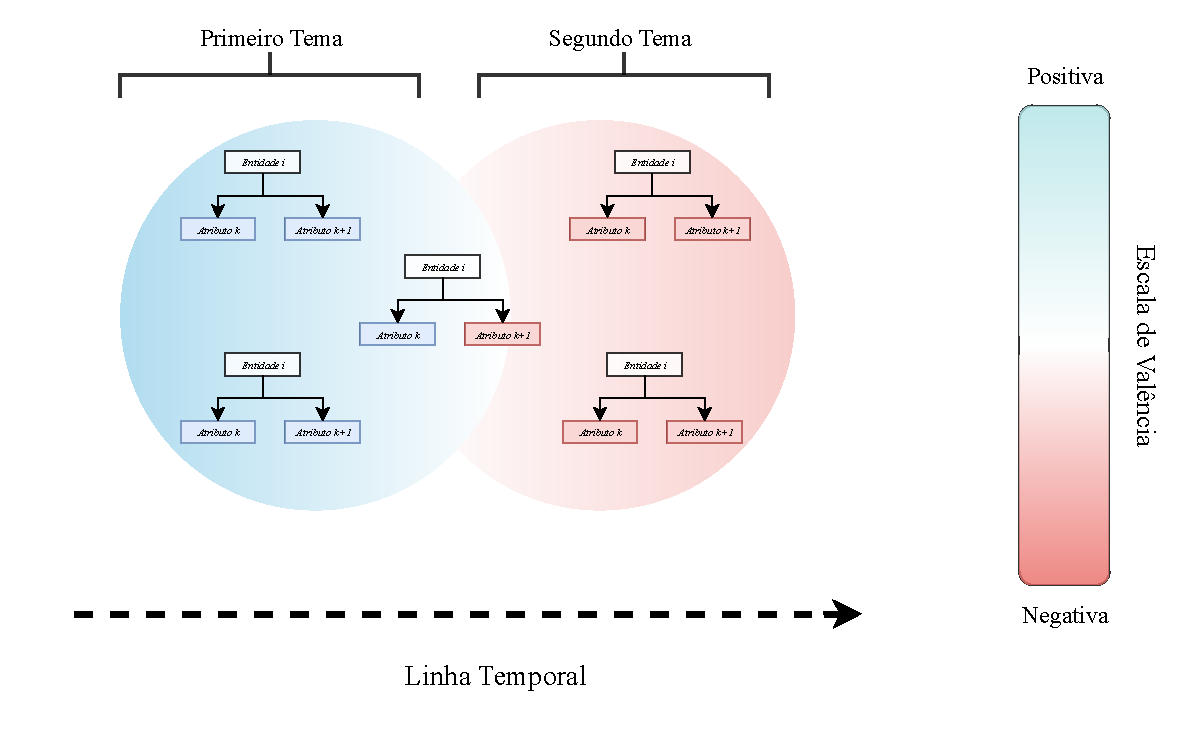
\includegraphics[width=1\linewidth]{figures/diagrama_discurso_autoritario}
\end{figure}

Figura 1 representa um diagrama simplicado do discurso político. A partir dele, pode-se compreender a dinâmica entre os elementos fundamentais e suas dimensões. Temas e Tempo ganham significado a medida em que um orador dispõem em sua fala setenças que conectam Atributos à Entidades. Uma vez que discursos políticos envolvem expressão de valor, espera-se que Atributos possuem uma polaridade -- positiva e negativa -- e que, por isso, funcionam como dispositivos para demarcar um posicionamento favorável ou desfavorável. Quanto mais Atributos negativos são utilizados para caracterizar as Entidades mencionadas sobre um tema, mais negativo será a compreensão geral da sentenças sobre o Tema.

Na Figura 1, as Entidades mencionadas no início do discurso tanto recebem atributos positivos como compartilham de uma atmosférica temática de maior valência. No outro extremo, as Entidades mencionadas ao final do discurso possuem o inverso dessas características -- Atributos e Tema e negativos. Portanto, pode-se inferir que, no escopo de Entidades do orador, seu posicionamento variou da simpatia manifesta no início da fala até a rejeição, ao final.

Um exemplo prático dessa dinâmica está presente nas contribuições de \citeonline{smith1990symptomology}. Nas falas de parlamentares analisadas pela autora, a expressão de rejeição à minorias apresentou dois modos típicos: i) a atribuição direta de características negativas e ii) o estabelecimento de uma correlação ilusória a partir da menção de Entidades em Temas carregados de polaridade negativa -- como crime, entorpecentes e problemas de incivilidade. Do ponto de vista dos ouvintes, um grupo social que compartilha um mesmo espaço semântico que elementos popularmente reprovados também é passível de estigma. De forma simétrica, a exaltação de Entidades associadas às autoridades se dá pelos mesmos mecanismos.

De forma, genérica, pode-se definir o nível de apoio de um parlamentar a uma Entidade em função da Valência dos Atributos (VA) e do Tema na qual ela é contextualizada. Na Equação 3.1, que especifica essa relação, é possível notar que o apoio a Entidade possui três componentes: dois que dizem respeito a atribuição direta de valor -- a Média da Valência dos Atributos (MVA) ponderada pela Saliência da Entidade (SE) -- e outro que refere-se a atribuição indireta -- Valência do Tema (VT).     

\begin{equation}
	SupEnt_i = \frac{\sum_{k = 1}^{K} VA_k}{K} * SA_i + VT_i
\end{equation}

\begin{equation}
SA_i = \frac{\sum_{q = 1}^{Q} Ent_q}{Q}
\end{equation}

\begin{equation}
VT_i = \frac{\sum_{p = 1}^{P} \sum_{j = 1}^{J} VA_{jp}}{P * J}
\end{equation}

Onde \emph{SupEnt} é o Apoio à Entidade que é função da \emph{VA} -- a Valência do Atributo \emph{k} associado a Entidade, da \emph{SA} -- que é a Saliência da Entidade, medida pela Frequência de menções a Entidade \emph{i} -- e da \emph{VT} -- que é a Valência do Tema, mensurada pela valência média dos \emph{J} atributos atribuídos por \emph{P} parlamentares a Entidades que integram o tema \emph{i}.

Alguns pontos relevantes de inferência são que, enquanto Média da Valência dos Atributos e a Saliência da Entidade dizem respeito a elementos controlados diretamente pelos oradores, a Valência do Tema é resultado da polaridade de todas as sentenças de todos os oradores sobre o Tema. Além disso, a Média da Valência dos Atributos de Entidades apresentam correlação proporcionalmente a distância temporal em que são mencionadas no discurso.  

A partir dos \emph{insights} levantados, pode-se tomar Apoio à Entidade como um instrumento para detecção da personalidade autoritária. Propõem-se, nessa investigação, que o Apoio à Entidades Subalternas e Apoio à Entidades Dominantes são medidas correlacionadas com as 3 dimensões do RWA: Agressividade Autoritária, Submissão Autoritária e Convencionalismo. Essas duas medidas são construídas a partir da estimativa do Apoio à Entidade -- segundo a Equação 3.1 -- de entidades textuais tipicamente associadas a i) populações subjugadas e ii) grupos e instituições dominantes.

Nas Equações 3.4 e 3.5, define-se, respectivamente, o Apoio à Entidades Subalternas como função do nível de Agressividade Autoritária do agente político, e, o Apoio à Entidades Dominantes, dos níveis de Submissão Autoritária e Convencionalismo. Ambas funções contém um termo estocástico cuja magnitude define o nível de ruído entre autoritarismo intrínseco e expresso.

\begin{equation}
SupEntMin = f(\theta_0 + \theta_1 * AuthAgress + u)
\end{equation}

\begin{equation}
SupEntDom = f(\tau_0 + \tau_1 * AuthSubmiss + \tau_2 * Convent + v)
\end{equation}

\subsection{Operacionalizando a Estimação dos Metaparâmetros}

Do ponto de vista da operacionabilidade do critério de classificação proposto, é necessário resolver o desafio de mensurar os parâmetros das funções que definem o Apoio à Entidades Dominantes e Subalternas. Para isso, algoritmos de inteligência artificial oferecem soluções para o problema. Em especial, serão utilizadas três técnicas que, respectivamente, i) identificam os tópicos principais de uma coleção de discursos, ii) reconhecem entidades textuais em uma sentença e iii) mensuram as valência de uma sentenção. São elas o LDA, NER (\emph{Named-Entity Recognition}) e Análise de Sentimentos.   



\chapter{Prova de Conceito: o caso da Câmara dos Deputados}\label{resultados}

\section{Coletando dados}

\section{Estimando meta-parâmetros textuais}

\section{Avaliando resultados}		
% ----------------------------------------------------------
% ELEMENTOS PÓS-TEXTUAIS
% ----------------------------------------------------------
\postextual
% ----------------------------------------------------------

% ----------------------------------------------------------
% Referências bibliográficas
% ----------------------------------------------------------
\bibliography{bibli}

% ----------------------------------------------------------
% Glossário
% ----------------------------------------------------------
%
% Consulte o manual da classe abntex2 para orientações sobre o glossário.
%
%\glossary

% ----------------------------------------------------------
% Apêndices
% ----------------------------------------------------------

Apêndices

%---------------------------------------------------------------------
% INDICE REMISSIVO
%---------------------------------------------------------------------
\phantompart
\printindex
%---------------------------------------------------------------------

\end{document}
